As described before, the experiment consisted of two phases, with three parts in total: the design of a training scenario, a grid search over the best hyperparameters, and the manoeuvres flown by the resulting controller. Although the training scenario design took place first, the resulting parameters came out of the settings found with the grid search. Therefore, this section presents the results of the three different experiment phases presented above in a slightly different order. First, the results of the hyperparameter search are presented. Those hyperparameters with the best performance were then used as a starting point for the training phase. Finally, the controller that was resulted from the training phase was saved, and the two test manoeuvres were performed by starting from the training save point. 

\subsection{Hyperparameter search} \label{ssec:results:training}
The grid search over the hyperparameters yielded two sets of results. Firstly, the success rate, defined as the percentage of trials that did not end prematurely, is shown in Fig. \ref{fig:training_params_success}. Trials could end prematurely in two ways: either by breaking the performance limits of $\pm90\si{\degree}$ in pitch and roll, or by "parameter explosion", which is numerical overflow of the neural network weights. Secondly, the final performance of the successful runs, measured in RMSE in the final ten seconds of successful trials, is shown in Fig. \ref{fig:training_params_rms}. 

\begin{figure}[th]
    \centering
    \subfloat[Success rates]{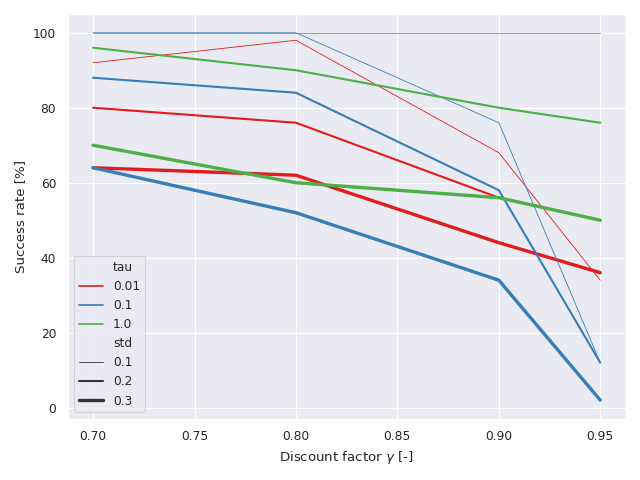
\includegraphics[width=0.45\textwidth]{fig/5/training/params_success.png} \label{fig:training_params_success}}
    \subfloat[Final performance]{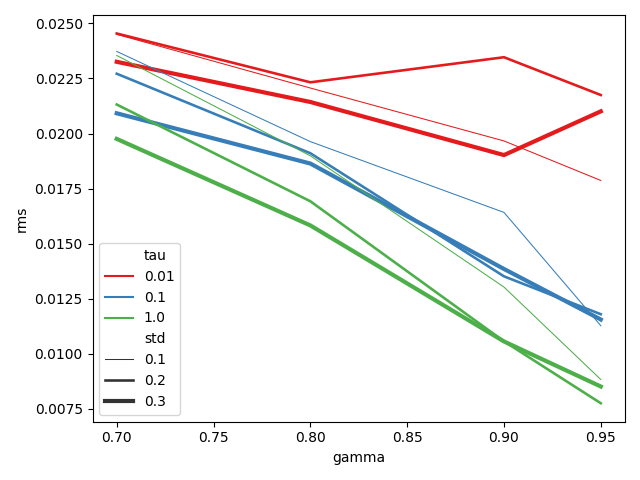
\includegraphics[width=0.45\textwidth]{fig/5/training/params_rms.png} \label{fig:training_params_rms}}
    \caption{Aggregated success rates and final performance of different combinations of training hyperparameters}
\end{figure}

Inspecting these figures, a few trends become visible. First, it can be seen that the discount factor $\gamma$ is simultaneously correlated with a lower success rate as well as higher final performance. This result exposes the "dual role" of the discount factor $\gamma$. As a discount factor explicitly weighs future rewards more or less strongly, it also implicitly serves as a variance reduction parameter, weighing the importance of the critic's estimate of value derivatives in the actor update. This makes a set-up with a low value of $\gamma$ less prone to the parameter explosion failure mode often found in ADP. On the other hand, a high value of $\gamma$ leads to stronger weighting of future rewards, which is important in tasks with relatively slow controls such as helicopter control. 
Secondly, in this implementation, higher values of $\tau$ were found to be correlated with both higher success rates and better final performance, all the way up to $\tau=1$. At $\tau=1$ the target critic immediately tracks the critic, and such is not used at all. This can be attributed to the fact that in this online learning scenario, the slow learning in presence of a target critic can actually cause the unstable helicopter environment to diverge more quickly than using a less robust but faster implementation without a target critic can. This was verified by comparing the failure modes with and without target critic: it was found that the majority of failures with a target critic in place were loss-of-control failures, while this shifted to numerical overflow failures when no target critic was in place. 
Thirdly, lower values of $\sigma_w$ were generally associated with higher success rates, but lower final performance. Based on these results, the hyperparameters used for training are shown in Fig. \ref{tab:training_end_hyperparams}. This combination showed a 100\% success rate in training over 100 random seeds while also having near-optimal final performance. 

\begin{table}[ht!]
\centering
\caption{Hyperparameters of the IDHP agents used in training}
\label{tab:training_end_hyperparams}
\begin{tabular}{@{}lll@{}}
\toprule
Hyperparameter               & Description                                 & Value \\ \midrule
$\gamma$                     & Discount factor                             & 0.95   \\
$\sigma_w$                   & Weight initialization standard deviation & 0.1   \\
$\tau$                       & Target critic mixing factor                 & 1.0  \\
$\eta^{lon}_{a} \; \eta^{lon}_c$ & Longitudinal agent actor and critic learning rates           & 5     \\
$\eta^{col}_{a} \; \eta^{col}_c $ & Collective agent learning rates             & 0.1   \\ \bottomrule
\end{tabular}
\end{table}

\subsection{Training phase}
A sample training episode is shown in Fig. \ref{fig:training_results}. It can be seen that both cyclic and collective are able to follow the reference signal after approximately ten seconds, after which the performance is slowly improved over the next 50 seconds. Around $t=90\si{\second}$, some yawing motion appears as the result of tail rotor saturation, which in return is the result of the collective approaching 90\% in low-speed flight. In the collective controller, it can be seen that manages to achieve two different steady-state (trim) points: even though the controller was initialized at the trim for 15$\si[per-mode=symbol]{\meter \per \second}$, it has no problem holding altitude at flight speeds as low as 2$\si[per-mode=symbol]{\meter \per \second}$.

\begin{figure}[htb!]
    \centering
    \subfloat[Tracking performance, control inputs and angular rates]{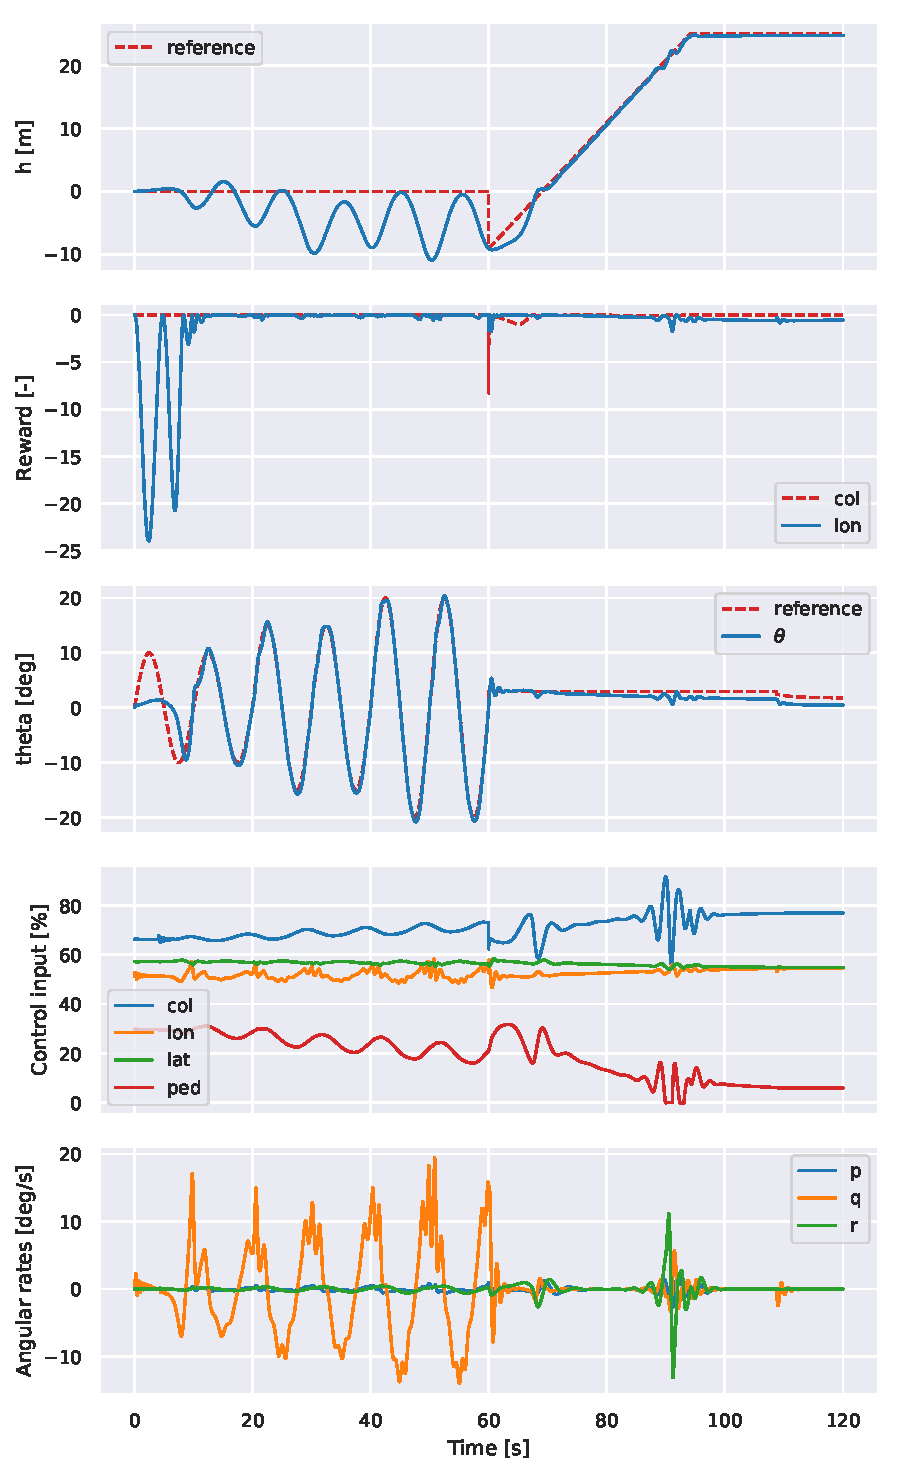
\includegraphics[width=0.48\textwidth]{fig/5/training/tracking.pdf} \label{fig:training_tracking}}
    \subfloat[Remaining state variables]{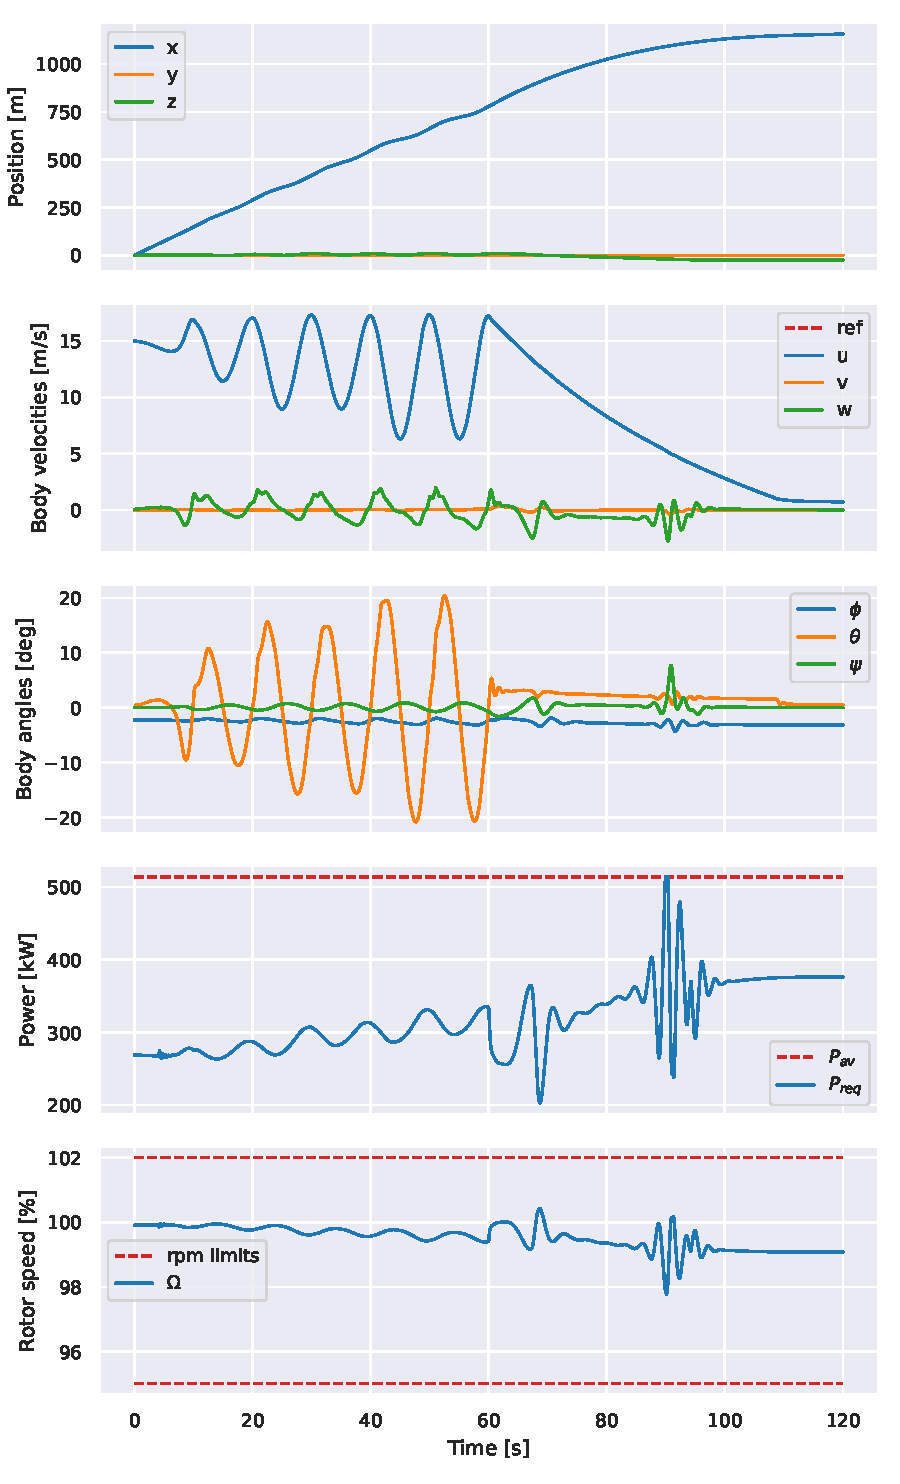
\includegraphics[width=0.48\textwidth]{fig/5/training/states.pdf} \label{fig:training_states}}
    \caption{Results of a sample training run}
    \label{fig:training_results}
\end{figure}

In Fig. \ref{fig:training_weights}, the learned parameters of the online estimated state and input matrices as well as the weights of both the actor and critic are shown. It can be seen that the parameters of both the state and input matrix in the incremental model converge within seconds, providing critical information to the actor and critic updates. 

\begin{figure}[htb]
    \centering
    \subfloat[Cyclic agent]{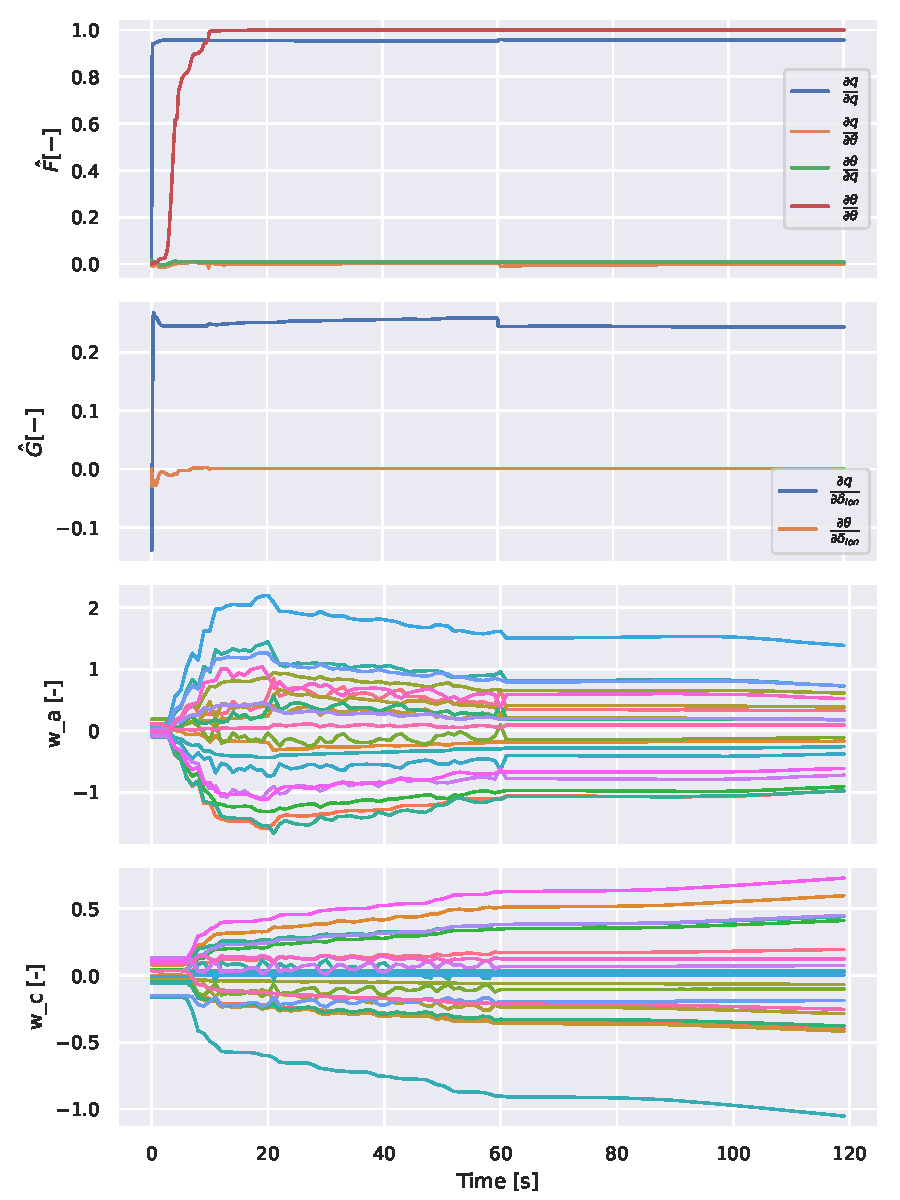
\includegraphics[width=0.48\textwidth]{fig/5/training/weights_cyclic.pdf} \label{fig:training_w_cyclic}}
    \subfloat[Collective agent]{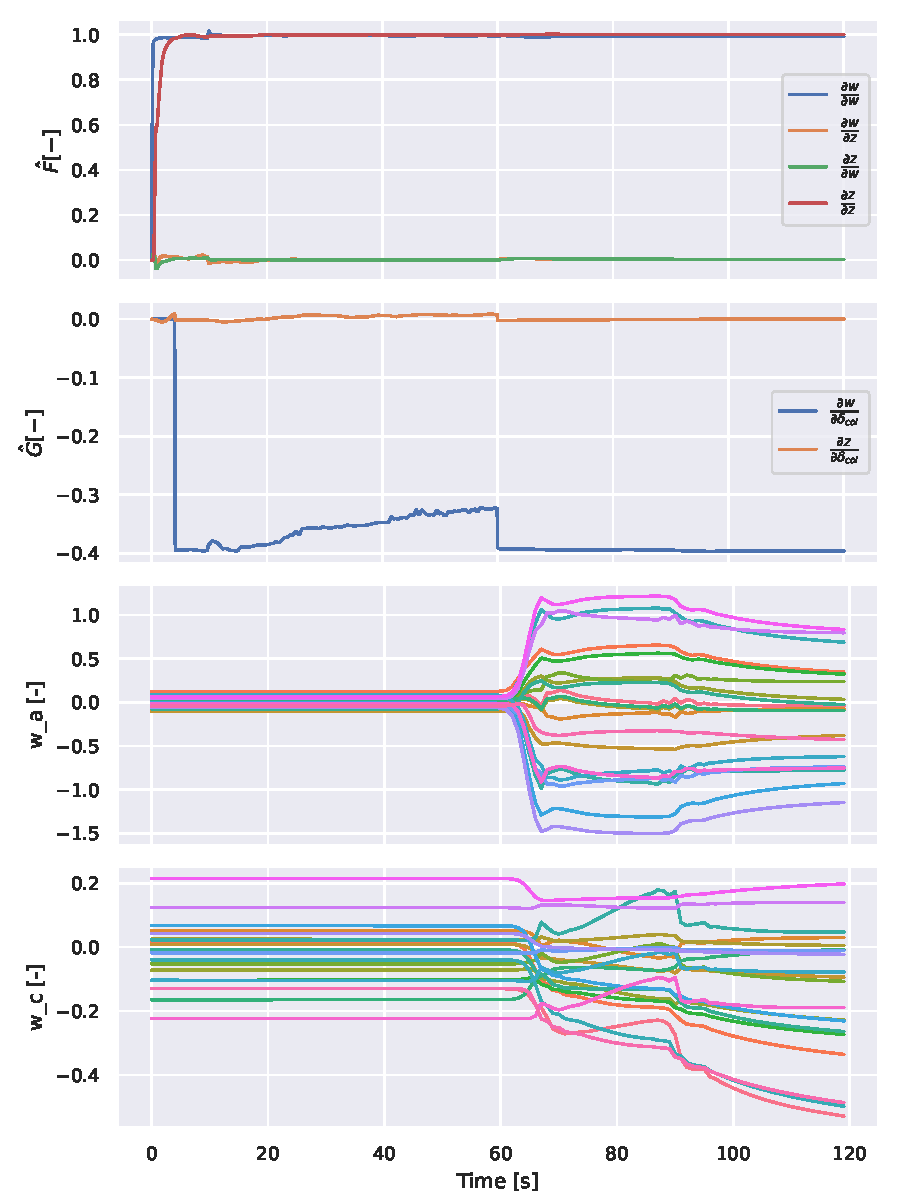
\includegraphics[width=0.48\textwidth]{fig/5/training/weights_collective.pdf} \label{fig:training_w_collective}}
    \caption{Estimates of the online identified incremental model, actor weights and critic weights during a sample training trial}
    \label{fig:training_weights}
\end{figure}

\subsection{Test phase} \label{ssec:results:test}
\subsubsection{Acceleration-deceleration}
% TODO: move legend in figure, add vertical lines  for flight phases
Fig. \ref{fig:results_acceldecel} shows the results of a successful episode from the proposed acceleration-deceleration test. In the figure, the different flight phases are indicated with numbered dashed vertical lines (NOTE NOT YET DONE). 
In phase 1, the helicopter is in hover. Some minor control excitation can be seen in the first second of the episode, as the environment in initialized in a slightly different state from saved agent. 

In phase 2, the helicopter starts accelerating from hover to $u=25\si[per-mode=symbol]{\meter \per \second}$. It can be seen that the actual forward velocity lags behind the commanded value quite significantly. The pitch angle reference is followed sharply in the sharp transient part of this phase, but is slightly above the reference during the second half of this phase. A slight altitude gain is also observed, though this is well within the limits of 15m. As a result of the high collective required for the acceleration, the pedal control saturates, leading to a slight yawing motion around $t = 8 \si{\second}$, which was the limiting factor in the aggressiveness of the manoeuvre. 

As soon at the required velocity is achieved, phase 3 starts and an aggressive pitch-up is performed to decelerate the helicopter. The leads to a sudden increase in altitude due to two reasons. Firstly, as the fuselage rotates from slightly pitched-down through the neutral position, the increases the vertical component of the thrust vector. Secondly, part of the lost kinetic energy of the helicopter is transferred to the main rotor, increasing the rotor speed to slightly below the maximum safe speed, which in turn increases the total thrust force. As a reaction to this, the collective is reduced significantly and the engine power is reduced to less than 5\%. The control system remains stable even with pitch rates over $40\si[per-mode=symbol]{\degree \per \second}$. The maximum pitch-up attitude of $24\si{\degree}$ is reached two seconds into the third phase. 

Throughout the episode, it can be observed that the reference pitch angle is smoothly tracked. The pitch angle does not reach the required $30\si{\degree}$ in the deceleration phase, as this would have led to large heading deviations due to pedal saturation. The maximum deviations in altitude, lateral track, and heading angle remain well within the performance bounds. 

The acceleration-deceleration did not meet all the desired performance standards of the ADS-33, as it was largely held back by collective-pedal coupling. This is likely a result of deficiencies in the helicopter model, which is rather simple. Similar trends were observed in \cite{VanDerVorst2001}. When compared to real-life test data, the trends of the control inputs were similar but the magnitude of the collective required was significantly smaller. 

\begin{figure}[htb]
    \centering
    \subfloat[Tracking performance, control inputs and angular rates]{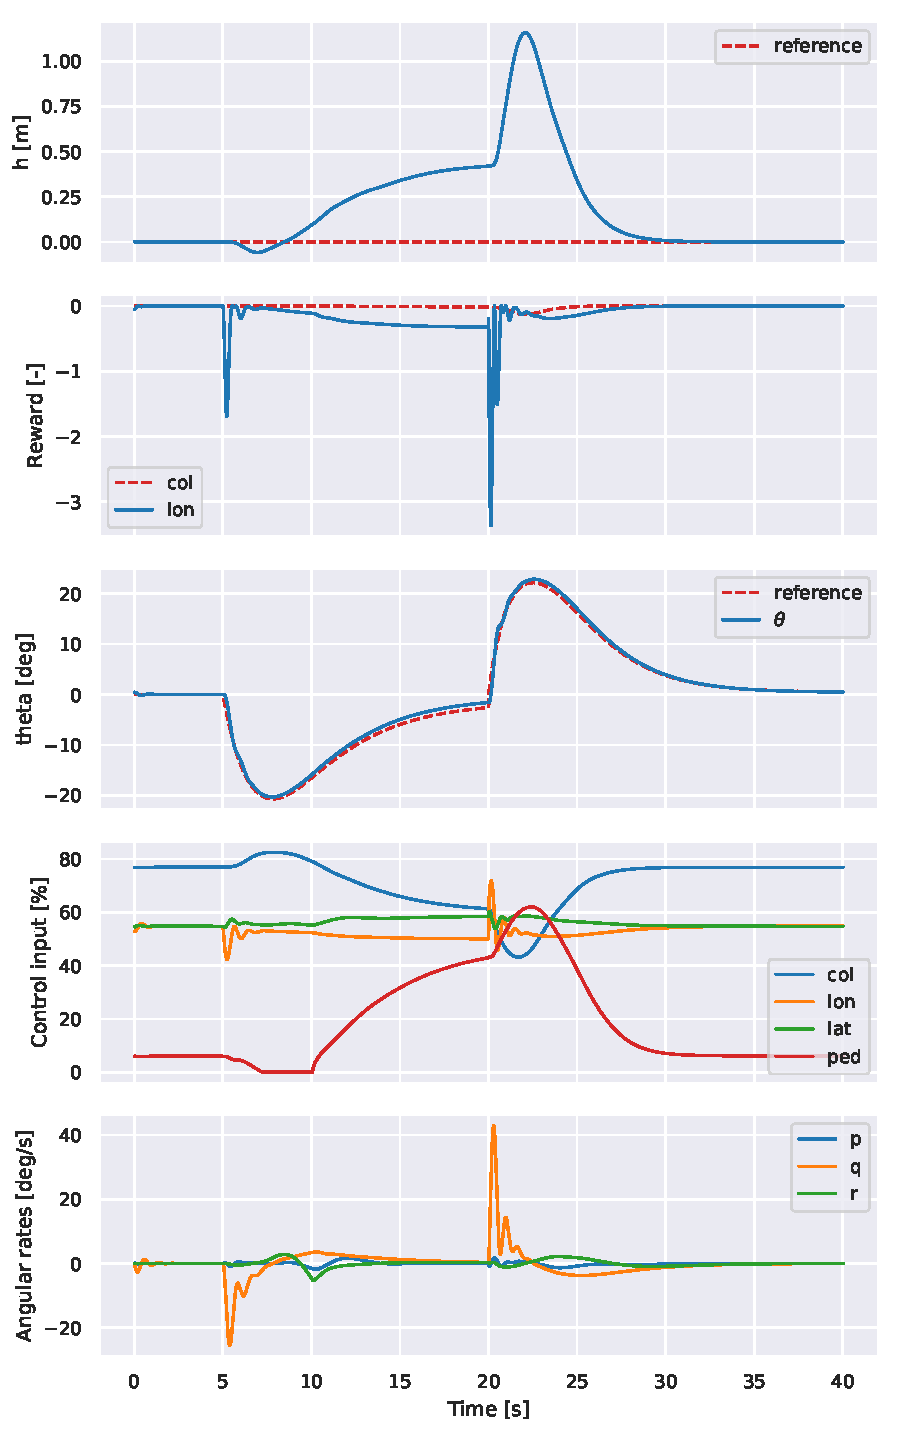
\includegraphics[width=0.48\textwidth]{fig/5/test/acdc/tracking.pdf} \label{fig:acdc_tracking}}
    \subfloat[Remaining state variables]{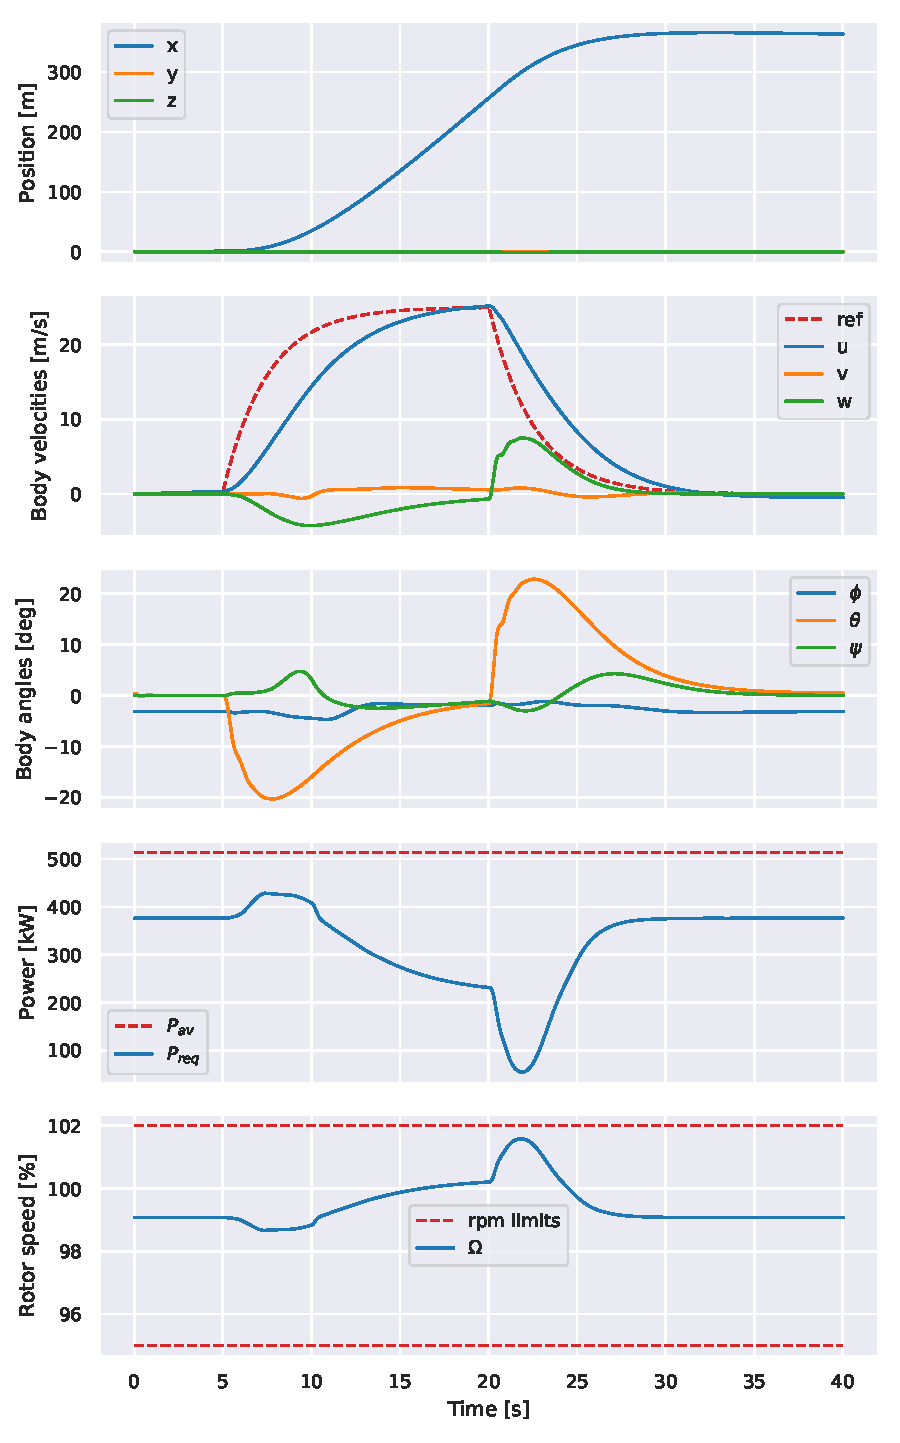
\includegraphics[width=0.48\textwidth]{fig/5/test/acdc/states.pdf} \label{fig:acdc_states}}
    \caption{Results of a sample run for the acceleration-deceleration test}
    \label{fig:results_acceldecel}
\end{figure}


\subsubsection{Continued landing}
The results of the continued landing test are shown in Fig. \ref{fig:results_landing}. 

In phase 1, a steady descending flight at a total airspeed of $V_{tas}=18\si[per-mode=symbol]{\meter \per \second}$ and a flight path angle $\gamma = -6\si{\degree}$ is performed. The agent, which was saved at approximately hover conditions, thus has to quickly establish a new approximate trim point. 

Phase 2 starts at $t=10\si{\second}$ when a single engine failure occurs, reducing the power available from the two-engine continuous limit $P_{aeo} = 514\si{\kilo\watt}$ to the single-engine transient limit $P_{oei,tr}=327\si{\kilo\watt}$. With a single engine the helicopter no longer has enough power to stop in a hover, requiring the performance of a continuous landing. However, in this steady descent phase, the engine is not performing at its limits, so nothing happens yet.

In phase 3, a flare is performed to reduce the forward airspeed as much as possible. The pitch angle reaches $17.6\si{\degree}$ when approximately $5\si{\meter}$ above the ground. To prevent the helicopter from losing too much altitude, the collective is also slightly increased while the forward airspeed is decreasing. The collective is then lowered and immediately increased to set in a slow descent with a reference vertical speed of $\dot{h}_{ref}=-0.5\si[per-mode=symbol]{\meter \per \second}$, while the cyclic is reduced to level out the airframe. As the forward airspeed decreases, the helicopter ends up in more and more of its own downwash, decreasing the efficiency and requiring more collective to keep the descent vertical speed stable. 

Phase 4 starts when the engine power reaches its maximum. As the engine power is insufficient to keep the descent steady, the collective is increased even further to trade rotor rotational speed for kinetic energy and cushion the last part of the landing. As a result, the helicopter touches down with forward and downward speeds of $u=3.11\si[per-mode=symbol]{\meter \per \second}$ and $w=0.82\si[per-mode=symbol]{\meter \per \second}$, which are both well within the safe values of 4.5$\si[per-mode=symbol]{\meter \per \second}$ and 1.5$\si[per-mode=symbol]{\meter \per \second}$, respectively. As the fourth phase lasted under five seconds, the choice for transient max power is warranted. Interestingly, it should be noted that the available power is likely underestimated as the ground effect is not taken into account in the simulation model. This would have increased the power available at these low speeds and altitudes, reducing the amount of rotor energy needed to cushion the landing. 

\begin{figure}[htb!]
    \centering
    \subfloat[Tracking performance, control inputs and angular rates]{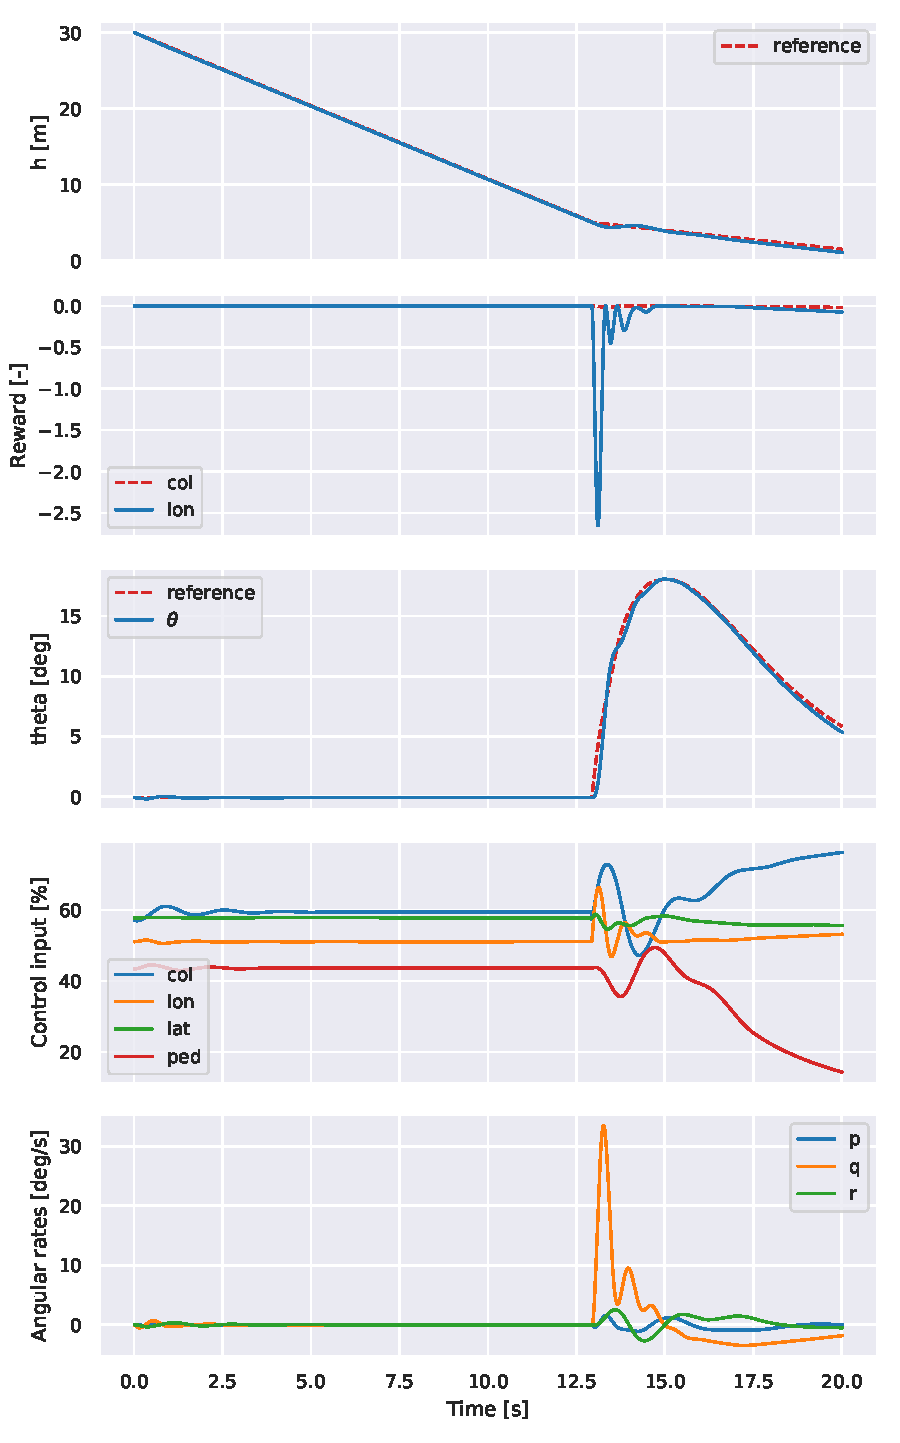
\includegraphics[width=0.48\textwidth]{fig/5/test/landing/tracking.pdf} \label{fig:land_tracking}}
    \subfloat[Remaining state variables]{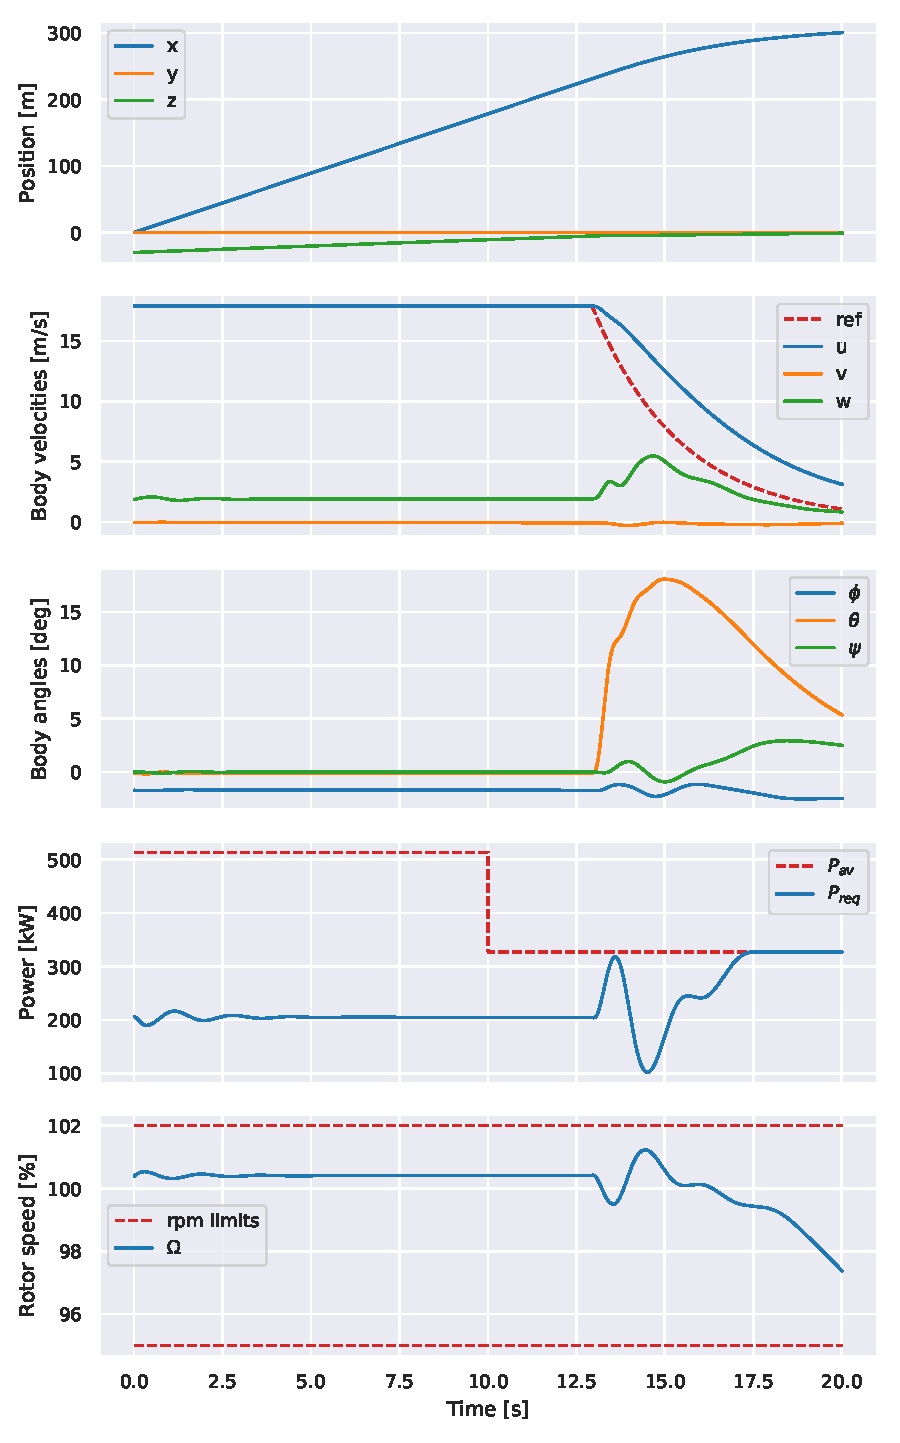
\includegraphics[width=0.48\textwidth]{fig/5/test/landing/states.pdf} \label{fig:land_states}}
    \caption{Results of a sample run for the landing test}
    \label{fig:results_landing}
\end{figure}

\FloatBarrier